\documentclass{article}

\usepackage[spanish]{babel}
\usepackage[numbers,sort&compress]{natbib}
\usepackage[T1]{fontenc}
\usepackage[ansinew]{inputenc}
\usepackage{graphicx}
\usepackage{url}

\title { Movimiento Browniano}
\author{Oscar Qui\~nonez}

\begin{document}

\maketitle
 
\section{Objetivo}\label{met}

A trav\'es de una simulaci\'on se intenta representar la manera en que el movimiento browniano afecta en el regreso de una part\'icula a su punto origen.

\section{Metodolog\'ia}\label{met}

Para llevar a cabo la simulaci\'on del movimiento browniano se utiliz\'o el programa R 4.0.2 para representar una caminata desde el origen, fueron simuladas hasta 8 dimensiones con los incrementos exponenciales entre 5 y 10, a cada incremento se le hicieron 50 repeticiones para conocer que tan probable podr\'ia ser el retorno al origen de la part\'icula. \cite{satuelisa} Fueron utilizadas las instrucciones de la tarea 1, \cite{clara} adem\'as del apoyo en el repositorio de Tellez, C.

\section{Resultados y Discusi\'on}\label{res}

Al realizar la simulaci\'on en R 4.0.2 se gener\'o una serie de datos que explican el regreso de la part\'icula al origen en cada una de las 8 dimensiones. A continuaci\'on se muestra la gr\'afica en la que se pueden ver las 8 dimensiones y como cada una de ellas esta representada por una columna. Ver figura 1.

\begin{figure}

 \begin{center}
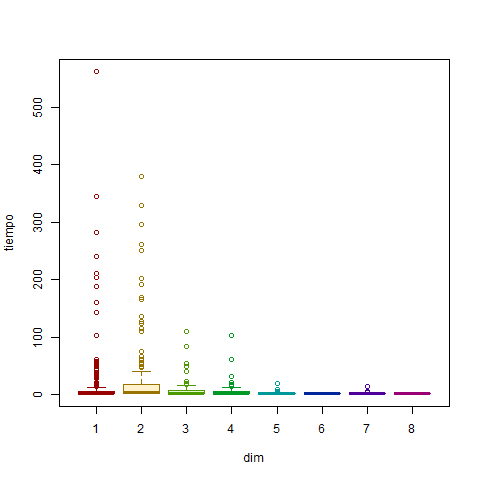
\includegraphics[scale=0.3]{demo.png}
\end{center}
  \caption{Tiempo para regresar al origen en cada una de las 8 dimensiones.}
  \label{f1}
 
\end{figure}
 
\newpage

\section{Conclusi\'on}

La simulaci\'on de modelos matem\'aticos usando R 4.0.2 nos ayud\'o a entender como una part\'icula regresa a su punto de origen en 8 dimensiones, se puede observar que mientras mas dimensiones recorra m\'as r\'apido regresa, pero al mismo tiempo es m\'as improbable que esto suceda. 

\bibliography{brownianotareauno}
\bibliographystyle{plainnat}


\end{document}